\chapter{بحر ديراك، وكتلة الفرميون، والسبينورات ذات الأربع مركبات}

\section{الفرميونات المتحركة إلى اليمين وبحر ديراك}

معادلة ديراك هي معادلة للفرميونات. أما البوزونات النسبية فتخضع لمعادلات مختلفة، مثل معادلة كلاين--غوردون أو معادلات ماكسويل. أبسط مثال يعيش في بعد مكاني واحد ويصف في البداية جسيمات وجسيمات مضادة لا يمكنها الحركة إلا إلى اليمين.

لنبدأ بموجة مستوية،
\begin{equation}
\psi(x,t)=\psi_0 e^{i(kx-\omega t)}.
\end{equation}
وسرعة طورها هي
\begin{equation}
v_{\mathrm{ph}}=\frac{\omega}{k}.
\end{equation}
وتهم إشارتا \(k\) و\(\omega\). فإذا كانتا متماثلتي الإشارة تحرك الطور إلى اليمين؛ وإذا كانتا متعاكستي الإشارة تحرك إلى اليسار. وعندما يكون \(\omega\) متناسبًا طرديًا مع \(k\)، تتطابق سرعتا الطور والمجموعة:
\begin{equation}
v_{\mathrm{g}}=\frac{d\omega}{dk}=\frac{\omega}{k}.
\end{equation}

اعتبر المعادلة من الرتبة الأولى
\begin{equation}
\frac{\partial\psi}{\partial x}
+
\frac{\partial\psi}{\partial t}
=0.
\end{equation}
بالتعويض بالموجة المستوية نحصل على
\begin{equation}
ik\psi-i\omega\psi=0,
\end{equation}
ومن ثم
\begin{equation}
\omega=k.
\end{equation}
ولذلك تتحرك الموجة إلى اليمين. ومن المفيد أن نوسم الحقل تبعًا لذلك:
\begin{equation}
\frac{\partial\psi_R}{\partial t}
=
-\frac{\partial\psi_R}{\partial x}.
\end{equation}

بإعادة إدخال سرعة الضوء نحصل على الصيغة ذات الأبعاد
\begin{equation}
\frac{\partial\psi_R}{\partial x}
+
\frac{1}{c}\frac{\partial\psi_R}{\partial t}
=0,
\end{equation}
بحيث
\begin{equation}
\omega=ck.
\end{equation}
ومن الآن فصاعدًا \(c=1\). ومع \(\hbar=1\)، تكون \(\omega\) أيضًا طاقة كم واحد.

\begin{figure}[htbp]
\centering
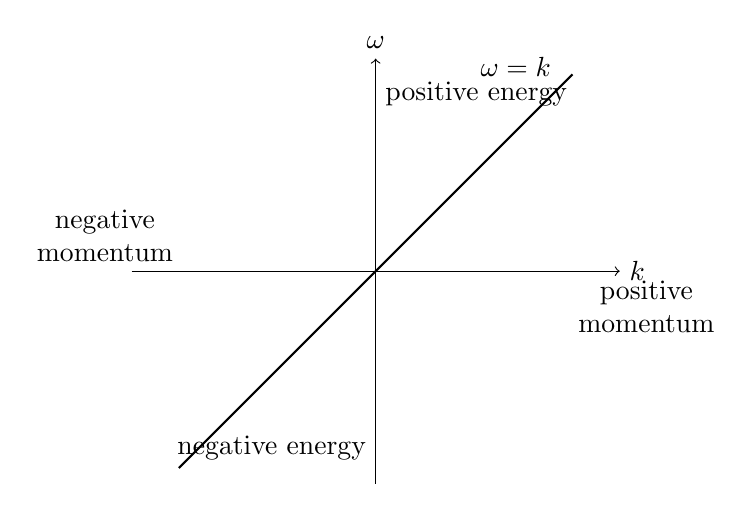
\begin{tikzpicture}[scale=1.0]
\draw[->] (-3.1,0) -- (3.1,0) node[right] {$k$};
\draw[->] (0,-2.7) -- (0,2.7) node[above] {$\omega$};
\draw[thick] (-2.5,-2.5) -- (2.5,2.5);
\node[above left] at (2.35,2.35) {$\omega=k$};
\node[below right,align=center] at (2.45,0) {positive\\momentum};
\node[above left,align=center] at (-2.45,0) {negative\\momentum};
\node[right] at (0,2.25) {positive energy};
\node[left] at (0,-2.25) {negative energy};
\end{tikzpicture}
\caption{تتضمن علاقة التشتت عديمة الكتلة للحركة إلى اليمين \(\omega=k\) فرعًا موجب الطاقة وآخر سالب الطاقة.}
\end{figure}

يترتب على هذا الخط المستقيم نتيجة خطيرة. فـ \(k\) الموجب يعطي طاقة موجبة، بينما يعطي \(k\) السالب طاقة سالبة. ومع ذلك يصف الجزآن موجات متحركة إلى اليمين لأن \(\omega/k=1\) على امتداد الخط كله.

يمكن لإلكترون موضوع على الجزء موجب الطاقة أن يهبط إلى حالة أدنى، ويبعث فوتونًا موجب الطاقة، ثم يهبط مرة أخرى، ويواصل النزول في الطيف: درجة ثم أخرى ثم أخرى. ولن يكون أي إلكترون مستقرًا. والأخطر من ذلك أن العالم سيخفض طاقته بإنتاج المزيد والمزيد من الإلكترونات سالبة الطاقة.

يوفر مبدأ الاستبعاد الفرميوني العلاج. املأ كل حالة إلكترونية سالبة الطاقة. فلا يمكن لإلكترون ثانٍ أن يدخل حالة مشغولة بالفعل، ولذلك فإن القطاع السالب الطاقة الممتلئ تمامًا يمنع هبوطًا غير محدود. وهذا القطاع الممتلئ هو بحر ديراك، وحالته الممتلئة تمامًا هي الحالة الأرضية، أو الفراغ.

\begin{classroomqa}
\lecturetimestamp{00:07:19}
\audiencequestion{هل توجد حالات أدنى سالبة الطاقة بعدد لا نهائي؟}
\lecturerresponse{نعم. إذا كانت الزخوم متقطعة كان الطيف أشبه بدرج لا نهائي؛ وإذا كانت مستمرة كان أشبه بمنحدر مستمر. إن ملء بحر الطاقة السالبة يمنع الإلكترون من الهبوط بلا نهاية، وإن كان انتقال هبوطي محدود مصحوب بإصدار فوتون قد يظل ممكنًا حين تتوافر حالة أدنى غير مشغولة.}
\end{classroomqa}

وهذا يفسر لماذا يجب أن تُكمم معادلة ذات هذا الطيف بوصفها نظرية فرميونية. فلو كانت الكمات بوزونات، لأمكن لعدد اعتباطي كبير منها أن يشغل الحالة الأدنى نفسها، ولما أدى ملء القطاع السالب الطاقة إلى استقرار الفراغ.

كما أن تصور البحر الممتلئ يولد جسيمات مضادة. ففي الفراغ تكون جميع المستويات سالبة الطاقة مشغولة، وجميع المستويات موجبة الطاقة فارغة. ويمكن رفع إلكترون من أي مستوى مشغول سالب الطاقة إلى أي مستوى فارغ موجب الطاقة؛ ولا يلزم أن يكون المستويان الابتدائي والنهائي موضوعين بتناظر.

\begin{figure}[htbp]
\centering
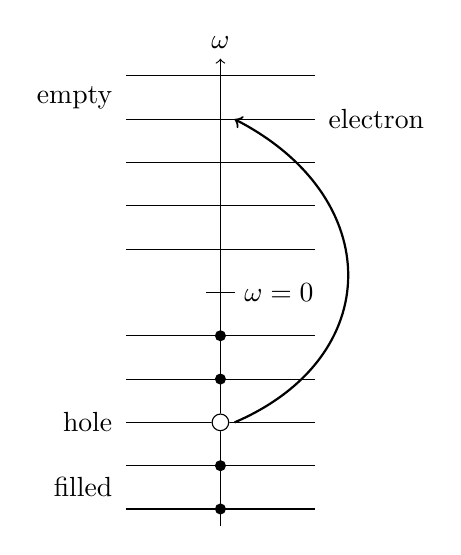
\begin{tikzpicture}[x=1cm,y=0.55cm]
\draw[->] (0,-5.4) -- (0,5.4) node[above] {$\omega$};
\draw (-0.18,0) -- (0.18,0) node[right] {$\omega=0$};
\foreach \y in {-5,-4,-3,-2,-1} {
  \draw (-1.2,\y) -- (1.2,\y);
  \fill (0,\y) circle (2pt);
}
\foreach \y in {1,2,3,4,5} {
  \draw (-1.2,\y) -- (1.2,\y);
}
\draw[->,thick] (0.18,-3) .. controls (2.1,-1.5) and (2.1,2.2) .. (0.18,4);
\draw[white,fill=white] (0,-3) circle (3pt);
\draw (0,-3) circle (3pt);
\node[left] at (-1.25,-3) {hole};
\node[left] at (-1.25,-4.5) {filled};
\node[left] at (-1.25,4.5) {empty};
\node[right] at (1.25,4) {electron};
\end{tikzpicture}
\caption{إن رفع إلكترون سالب الطاقة من مستوى مشغول يُنتج إلكترونًا موجب الطاقة ويترك فجوة في البحر الممتلئ.}
\end{figure}

إن إزالة إلكترون ذي طاقة سالبة ترفع الطاقة بالنسبة إلى الفراغ، ولذا تكون للفجوة طاقة موجبة. وعلى الفرع \(\omega=k\)، كان الإلكترون المنزوع ذا زخم سالب أيضًا. وإزالة زخم سالب تترك فائضًا موجبًا من الزخم، ولذا يكون للفجوة زخم موجب. وإذا اعتبرنا شحنة الإلكترون سالبة، فإن الإلكترون المفقود تكون شحنته موجبة. وهكذا تكون الفجوة جسيمًا مضادًا موجب الطاقة موجب الزخم، بينما يكون الإلكترون المرفوع ذا شحنة سالبة وطاقة موجبة وزخم موجب. وكل إثارة حقيقية في هذه النظرية ذات الفرع الواحد تتحرك إلى اليمين.

يُبنى الحقل \(\psi_R\) من مؤثرات إنشاء وفناء فرميونية. ولذلك فإن تفسير الجسيم والفجوة هو وصف للكمات التي ينشئها الحقل ويزيلها، لا لموجة كلاسيكية فقط.

ولا يزال هناك عدم تناظر. فالبحر المتحرك إلى اليمين يحتوي على حالات سالبة الطاقة ذات زخم سالب. وزخمه الكلي الصوري هائل ويتجه إلى اليسار. ويمكن تعريف زخم الفراغ على أنه صفر بطرح ذلك الثابت، لكن الحالة تبقى غير متوازنة بنيويًا: فالجسيمات والجسيمات المضادة تتحرك إلى اليمين فقط، بينما يتكوّن الفراغ الممتلئ من حالات ذات زخم سالب.

\section{الفرع المتحرك إلى اليسار وفراغ متوازن}

يتطلب التوازن بين اليسار واليمين حقلاً ثانيًا مستقلًا له مؤثراته الخاصة للإنشاء والفناء. ولنفرض أنه يحقق
\begin{equation}
\frac{\partial\psi_L}{\partial t}
=
+\frac{\partial\psi_L}{\partial x}.
\end{equation}
ولصيغة الموجة المستوية نفسها،
\begin{equation}
-i\omega\psi_L=ik\psi_L,
\end{equation}
ومن ثم
\begin{equation}
\omega=-k.
\end{equation}
وهذا الخط الثاني هو الصورة المرآتية لـ \(\omega=k\). ويصف فرعه موجب الطاقة جسيمات متحركة إلى اليسار، ويجب أيضًا ملء فرعه سالب الطاقة.

\begin{figure}[htbp]
\centering
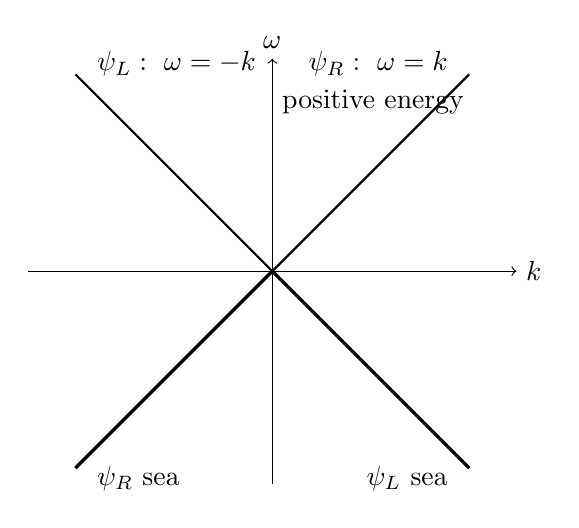
\begin{tikzpicture}[scale=1.0]
\draw[->] (-3.1,0) -- (3.1,0) node[right] {$k$};
\draw[->] (0,-2.7) -- (0,2.7) node[above] {$\omega$};
\draw[thick] (-2.5,-2.5) -- (2.5,2.5);
\draw[thick] (-2.5,2.5) -- (2.5,-2.5);
\draw[very thick] (-2.5,-2.5) -- (0,0);
\draw[very thick] (0,0) -- (2.5,-2.5);
\node[above left] at (2.35,2.35) {$\psi_R:\ \omega=k$};
\node[above right] at (-2.35,2.35) {$\psi_L:\ \omega=-k$};
\node[right] at (0,2.15) {positive energy};
\node[below right] at (-2.35,-2.35) {$\psi_R$ sea};
\node[below left] at (2.35,-2.35) {$\psi_L$ sea};
\end{tikzpicture}
\caption{يعطي الحقلان المستقلان المتحركان إلى اليمين وإلى اليسار فرعين عديمي الكتلة متقابلين مرآتيًا؛ ويُملأ في الفراغ النصفان السالبا الطاقة منهما.}
\end{figure}

بعد ملء بحري الطاقة السالبة كليهما، يصبح عدد الحالات المشغولة المتحركة إلى اليسار مساويًا لعدد نظيراتها المتحركة إلى اليمين. وتتوازن زخومهما في الفراغ. ويمكن الآن لإثارات الجسيمات والفجوات أن تتحرك في أي من الاتجاهين.

\begin{classroomqa}
\lecturetimestamp{00:15:58}
\audiencequestion{هل يمكن معالجة مشكلة الطاقة السالبة من دون افتراض حالات ممتلئة وفجوات؟}
\lecturerresponse{يمكن إعادة تسمية النظرية نفسها. فقد تُسمّى حالة إلكترون ممتلئة سالبة الطاقة حالةَ جسيم مضاد فارغة؛ وعندئذ لا تحتوي اللغة الفيزيائية إلا على جسيمات وجسيمات مضادة موجبة الطاقة. ومع ذلك يظل تصور البحر الممتلئ أداة مفيدة للتحقق من الاتساق، على غرار نطاق ممتلئ في معدن، حيث تؤدي إزالة إلكترون إلى توليد فجوة، بينما يؤدي رفعه إلى توليد جسيم وفجوة معًا.}
\end{classroomqa}

الإثارات التي نوقشت حتى الآن عديمة الكتلة. فعلاقات تشتتها خطية، ومقادير سرعاتها هي \(1\)، لذا فإنها تتحرك بسرعة الضوء. والسؤال التالي هو كيف نمنحها كتلة.

\section{مركبتان وحد الكتلة}

أولًا نجمع الحقلين في عمود:
\begin{equation}
\Psi=
\begin{pmatrix}
\psi_R\\
\psi_L
\end{pmatrix}.
\end{equation}
وهذا في البداية ليس إلا ترميزًا مضغوطًا لمعادلتين مستقلتين. عرّف
\begin{equation}
\alpha=
\begin{pmatrix}
1&0\\
0&-1
\end{pmatrix}.
\end{equation}
فتصبح معادلتا الحركة إلى اليمين وإلى اليسار
\begin{equation}
\frac{\partial\Psi}{\partial t}
=
-\alpha\frac{\partial\Psi}{\partial x}.
\end{equation}

\begin{figure}[htbp]
\centering
\includegraphics[width=0.78\textwidth]{lecture_06_figure_02.png}
\caption{يشكل الحقلان \(\psi_R\) و\(\psi_L\) سبينورًا ذا مركبتين، وتميز \(\alpha\) الفرعين العديمي الكتلة.}
\lectureframe{00:20:36}
\end{figure}

بالنسبة إلى موجة مستوية، فإن المؤثرين
\begin{equation}
i\partial_t
\quad\hbox{and}\quad
-i\partial_x
\end{equation}
يعطيان \(\omega\) و\(k\)، على الترتيب. ولذلك يمكن اختصار المعادلة المصفوفية إلى
\begin{equation}
\omega=\alpha k.
\end{equation}
وبالنسبة إلى المركبة العليا فهذا يعني \(\omega=k\)؛ وبالنسبة إلى المركبة السفلى يعني \(\omega=-k\). لقد اختزل هذا الترميز المعادلتين، لكنه لم يدخل أي فيزياء جديدة.

الإلكترونات ليست عديمة الكتلة ولا تتحرك بسرعة الضوء. ومن المغري أن نكتب لطاقة الإلكترون صيغة الطاقة الحركية اللانسبية \(k^2/(2m)\)، لكن ذلك لا يمكن أن يكون نقطة البداية هنا: فالحد عديم الكتلة يتعلق أصلًا بحركة بسرعة الضوء. والعلاقة النسبية هي
\begin{equation}
\omega^2=k^2+m^2,
\end{equation}
أو، مع تضمين فرعي الطاقة كليهما،
\begin{equation}
\omega=\pm\sqrt{k^2+m^2}.
\end{equation}
وعندما يكون \(m=0\)، تختزل هاتان العلاقتان إلى \(\omega=k\) و\(\omega=-k\).

\begin{classroomqa}
\lecturetimestamp{00:25:23}
\audiencequestion{هل تُستخدم وحدات يكون فيها \(c=1\)، وكيف تُستخرج سرعة جسيم ذي كتلة؟}
\lecturerresponse{نعم. سرعة الحزمة الموجية هي سرعة المجموعة، \(v_{\mathrm g}=d\omega/dk=k/\sqrt{k^2+m^2}\) على فرع الطاقة الموجبة. ومن ثم فإن علاقة التشتت نفسها تتضمن انخفاض السرعة إلى ما دون \(c=1\) لجسيم ذي كتلة.}
\end{classroomqa}

\begin{classroomqa}
\lecturetimestamp{00:26:29}
\audiencequestion{هل \(\omega\) متجه أم مصفوفة في الصياغة المختصرة \(\omega=\alpha k\)؟}
\lecturerresponse{تمثل هذه الصياغة المختصرة معادلة مؤثرات تؤثر في دالة الموجة ذات المركبتين. فهنا تعني \(\omega\) المقدار \(i\partial_t\)، وتعني \(k\) المقدار \(-i\partial_x\)، و\(\alpha\) هي المصفوفة التي تؤثر في فهرس المركبة. ولا يصبح الرمزان القياسيان \(\omega\) و\(k\) قيمتيهما الذاتيتين العدديتين إلا على موجة مستوية.}
\end{classroomqa}

أبق المعادلة من الرتبة الأولى، وجرّب أبسط امتداد يعتمد على الكتلة:
\begin{equation}
\omega=\alpha k+\beta m.
\end{equation}
ويجب أن يكون \(\beta\) مصفوفة، لأنه يؤثر في الحقل نفسه ذي المركبتين الذي يؤثر فيه \(\alpha\). ويمكن استنتاج جبره من تربيع المعادلة:
\begin{align}
\omega^2
&=(\alpha k+\beta m)(\alpha k+\beta m)\\
&=\alpha^2k^2+\beta^2m^2
+\alpha\beta\,km+\beta\alpha\,mk\\
&=\alpha^2k^2+\beta^2m^2
+(\alpha\beta+\beta\alpha)km.
\end{align}
وللحصول على \(k^2+m^2\) لكل \(k\) و\(m\)، نطلب
\begin{equation}
\alpha^2=I,
\qquad
\beta^2=I,
\qquad
\alpha\beta+\beta\alpha=0.
\end{equation}

لا يمكن لعددين عاديين غير صفريين أن يحققا الشرط الأخير: ففي حالة الأعداد سنحصل على \(2\alpha\beta=0\)، مع أن مربعيهما كلاهما يساوي \(1\). أما المصفوفات فيمكنها أن تحقق تبادلاً تضاديًا. وعلى وجه الخصوص، لا يمكن أن يكون \(\beta\) مساويًا لـ \(\alpha\)، لأننا عندئذٍ نحصل على
\begin{equation}
\alpha\beta+\beta\alpha=2\alpha^2=2I.
\end{equation}

اختر
\begin{equation}
\beta=
\begin{pmatrix}
0&1\\
1&0
\end{pmatrix}.
\end{equation}
ويمكن التحقق من مربعه عنصرًا عنصرًا:
\begin{equation}
\begin{aligned}
\beta^2
&=
\begin{pmatrix}
0&1\\
1&0
\end{pmatrix}
\begin{pmatrix}
0&1\\
1&0
\end{pmatrix}\\
&=
\begin{pmatrix}
0\cdot0+1\cdot1&0\cdot1+1\cdot0\\
1\cdot0+0\cdot1&1\cdot1+0\cdot0
\end{pmatrix}
=
\begin{pmatrix}
1&0\\
0&1
\end{pmatrix}.
\end{aligned}
\end{equation}
وترتيب الضرب مهم:
\begin{align}
\alpha\beta
&=
\begin{pmatrix}
1&0\\
0&-1
\end{pmatrix}
\begin{pmatrix}
0&1\\
1&0
\end{pmatrix}
=
\begin{pmatrix}
0&1\\
-1&0
\end{pmatrix},\\
\beta\alpha
&=
\begin{pmatrix}
0&1\\
1&0
\end{pmatrix}
\begin{pmatrix}
1&0\\
0&-1
\end{pmatrix}
=
\begin{pmatrix}
0&-1\\
1&0
\end{pmatrix}.
\end{align}
ومن ثم
\begin{equation}
\alpha\beta=-\beta\alpha,
\qquad
\alpha\beta+\beta\alpha=0.
\end{equation}
وتوجد اختيارات مصفوفية أخرى مكافئة، لكن هذا الاختيار يجعل معادلات المركبتين واضحة على نحو خاص.

إن إعادة مؤثرات التفاضل تعطي المعادلة ذات الكتلة
\begin{equation}
i\frac{\partial\Psi}{\partial t}
=
-i\alpha\frac{\partial\Psi}{\partial x}
+m\beta\Psi.
\end{equation}
وتبدّل المصفوفة \(\beta\) المركبتين:
\begin{equation}
\beta
\begin{pmatrix}
\psi_R\\
\psi_L
\end{pmatrix}
=
\begin{pmatrix}
\psi_L\\
\psi_R
\end{pmatrix}.
\end{equation}
وبناءً على ذلك،
\begin{align}
i\dot{\psi}_R
&=-i\frac{\partial\psi_R}{\partial x}+m\psi_L,\\
i\dot{\psi}_L
&=+i\frac{\partial\psi_L}{\partial x}+m\psi_R.
\end{align}

يقرن حد الكتلة بين حقول كانت مستقلة في النظرية عديمة الكتلة. فمعادلة المركبة العليا تتضمن المركبة السفلى، ومعادلة المركبة السفلى تتضمن المركبة العليا. وهذا الاقتران هو المقصود بكتلة ديراك. والمعادلات ثابتة تحت الانتقالات، لذا فهي تحفظ الزخم، وكتلة إثاراتها الجسيمية هي \(m\).

\begin{classroomqa}
\lecturetimestamp{00:38:25}
\audiencequestion{هل يكون الحل تلقائيًا ثابتًا تحت تحولات لورنتز؟}
\lecturerresponse{لا ينبغي أن يبقى حل بعينه ثابتًا تحت تحويل لورنتز. فالحالة ذات زخم معين تُحوَّل إلى حالة ذات الزخم المتحوَّل، لذا فالعبارة المناسبة هي التغايرية. والعلاقة \(\omega^2=k^2+m^2\) هي أحد الفحوص الأساسية الثابتة لورنتزيًا، لكن التغايرية التامة تتطلب أيضًا قانون تحول السبينور \(\Psi\)، وهو ما لم يُثبَت بعد.}
\end{classroomqa}

\section{إطار السكون ومعنى المركبتين}

لا يمكن إحضار جسيم عديم الكتلة إلى السكون، لكن يمكن ذلك لجسيم ذي كتلة. في السكون يكون \(k=0\)، ولذلك لا يكون للدالة الموجية أي تغير مكاني و
\begin{equation}
\omega=\beta m.
\end{equation}
وتختزل المعادلة التفاضلية إلى
\begin{equation}
i\frac{d\Psi}{dt}=m\beta\Psi.
\end{equation}
وبالمركبتين،
\begin{align}
i\dot{\psi}_R&=m\psi_L,\\
i\dot{\psi}_L&=m\psi_R.
\end{align}
وكلتا المدخلتين خارج القطر في \(\beta\) هما \(+1\)، لذا لا توجد إشارة سالب إضافية في أي من هاتين المعادلتين.

تنفصل المعادلتان بعد جمع المركبتين وطرحهما. عرّف
\begin{equation}
\psi_+=\psi_R+\psi_L,
\qquad
\psi_-=\psi_R-\psi_L.
\end{equation}
إن جمع معادلتي إطار السكون يعطي
\begin{equation}
i\dot{\psi}_+=m\psi_+,
\end{equation}
بينما يعطي طرحهما
\begin{equation}
i\dot{\psi}_-=-m\psi_-.
\end{equation}
ومن ثم
\begin{equation}
\omega=+m
\quad\hbox{for }\psi_+,
\qquad
\omega=-m
\quad\hbox{for }\psi_-.
\end{equation}

\begin{figure}[htbp]
\centering
\includegraphics[width=0.62\textwidth]{lecture_06_figure_03.png}
\caption{عند الزخم الصفري، يكون لـ \(\psi_+=\psi_R+\psi_L\) و\(\psi_-=\psi_R-\psi_L\) ترددا السكون \(\omega=+m\) و\(\omega=-m\).}
\lectureframe{00:44:49}
\end{figure}

الحقل الساكن ذو الطاقة الموجبة هو \(\psi_+\)؛ والحقل الساكن ذو الطاقة السالبة هو \(\psi_-\). وحالات الطاقة السالبة ممتلئة، كما من قبل. ونتيجة إطار السكون ليست إلا المقطع \(k=0\) من الطيف الكامل:
\begin{equation}
\omega_\pm(k)=\pm\sqrt{k^2+m^2}.
\end{equation}
\begin{figure}[htbp]
\centering
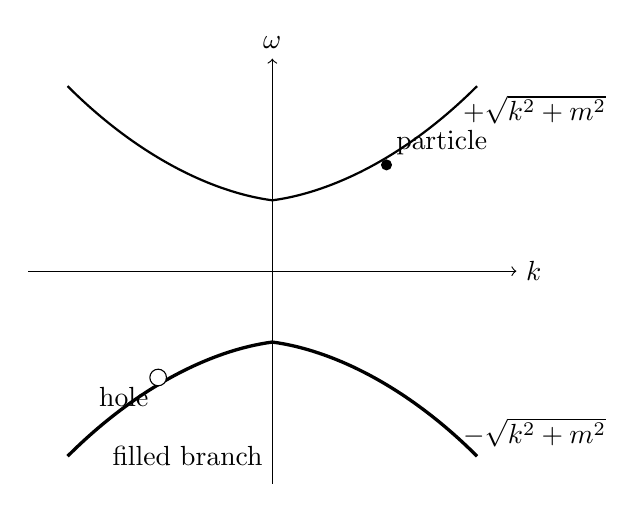
\begin{tikzpicture}[scale=1.0]
\draw[->] (-3.1,0) -- (3.1,0) node[right] {$k$};
\draw[->] (0,-2.7) -- (0,2.7) node[above] {$\omega$};
\draw[thick] (-2.6,2.35)
  .. controls (-1.7,1.45) and (-0.75,1.0) .. (0,0.9)
  .. controls (0.75,1.0) and (1.7,1.45) .. (2.6,2.35);
\draw[very thick] (-2.6,-2.35)
  .. controls (-1.7,-1.45) and (-0.75,-1.0) .. (0,-0.9)
  .. controls (0.75,-1.0) and (1.7,-1.45) .. (2.6,-2.35);
\fill (1.45,1.35) circle (2pt);
\node[above right] at (1.45,1.35) {particle};
\fill[white] (-1.45,-1.35) circle (3pt);
\draw (-1.45,-1.35) circle (3pt);
\node[below left] at (-1.45,-1.35) {hole};
\node[right] at (2.3,2.05) {$+\sqrt{k^2+m^2}$};
\node[right] at (2.3,-2.05) {$-\sqrt{k^2+m^2}$};
\node[left] at (0,-2.35) {filled branch};
\end{tikzpicture}
\caption{عند كل زخم، يحوي الطيف ذو الكتلة حالات ذات طاقة موجبة وأخرى ذات طاقة سالبة. والفرع السالب ممتلئ، والحالة المفقودة فيه هي ثقب ذو طاقة موجبة.}
\end{figure}
لكل زخم حالة ذات طاقة موجبة وحالة ذات طاقة سالبة. ويؤدي ملء كل حالة على الفرع السالب إلى جسيمات ذات طاقة موجبة فوق البحر وثقوب ذات طاقة موجبة فيه. ولكل من الجسيمات والثقوب كتلة موجبة.

تستحق النقطة الأساسية أن تُكرَّر. يصبح الفرميون ذا كتلة عندما تُقرن مركبتاه اللتان كانتا مستقلتين سابقًا. وفي السكون، لا تكون أي من المركبتين الأصليتين وحدها حالة ذاتية للطاقة. أما الحالات ذات الطاقة المحددة فهي مجموعهما وفرقُهما.

ولرؤية ما يعنيه المجموع، لِنرمز بـ \(C_R^\dagger\) و\(C_L^\dagger\) إلى مؤثري الخلق المعنيين للجسيم الواحد. فإن التأثير في الفراغ بـ
\begin{equation}
(C_R^\dagger+C_L^\dagger)\lvert0\rangle
\end{equation}
يُنشئ جسيمًا واحدًا في تراكب متماسك للمركبتين. وهو لا يُنشئ جسيمين. أما حاصل الضرب،
\begin{equation}
C_R^\dagger C_L^\dagger\lvert0\rangle,
\end{equation}
فيحتوي على مؤثري خلق ويُنشئ حالة ذات جسيمين عندما يكون كلا النمطين متاحًا. وبعد التطبيع، تكون احتمالية حالة السكون متساوية في المركبتين، لكن الموجة المقترنة ككل لها زخم صفري.

كان الوسمان \(R\) و\(L\) يشيران حرفيًا إلى الحركة فقط عندما \(m=0\). وما إن يوجد حد الكتلة، فإن الحل المتحرك ذي الكتلة يحتوي عمومًا على كلتا المركبتين، كما أن حل السكون يحتويهما بمقدار متساوٍ. ولذلك فمن الأفضل هنا النظر إلى \(R\) و\(L\) على أنهما وسمان للمركبتين العليا والسفلى للسبينور.

\begin{figure}[htbp]
\centering
\includegraphics[width=0.78\textwidth]{lecture_06_figure_04.png}
\caption{عندما تكون الكتلة غير منعدمة، تكون مركبتا السبينور مقترنتين؛ ولا ينطبق تفسيرهما بوصفهما متحركتين يمينًا ويسارًا مباشرة إلا في الحد العديم الكتلة.}
\lectureframe{00:50:48}
\end{figure}

تُبنى جميع الفرميونات ذات الكتلة في فيزياء الجسيمات من حقول ذات مركبة يسرى وأخرى يمنى: فكتلة ديراك تقرن بين مركبات تكون مستقلة في الحد العديم الكتلة.

\begin{classroomqa}
\lecturetimestamp{00:52:01}
\audiencequestion{هل ينبغي أن يتضمن \(\psi_R\pm\psi_L\) عاملًا مقداره \(1/\sqrt{2}\)؟}
\lecturerresponse{يمكن تضمينه لتطبيع الحالة. فهو يضرب طرفي المعادلة، ولذلك لا يغير معادلة الحركة.}
\end{classroomqa}

\begin{classroomqa}
\lecturetimestamp{00:52:12}
\audiencequestion{هل تهم المقادير النسبية للمركبتين اليمنى واليسرى؟}
\lecturerresponse{بالنسبة إلى الحالات الذاتية المختارة في إطار السكون، فإن مقداريهما متساويان. أما التطبيع الكلي فاعتباطي، لكن المقادير النسبية يحددها المتجه الذاتي لـ \(\beta\).}
\end{classroomqa}

\begin{classroomqa}
\lecturetimestamp{00:52:52}
\audiencequestion{هل يمكن أن يكون بين المركبتين طور نسبي؟}
\lecturerresponse{نعم. تنشأ المعاملات الحقيقية في \(\psi_R\pm\psi_L\) من اختيار \(\beta\) حقيقي. وتوجد اختيارات مكافئة أخرى لمصفوفات مربعها مصفوفة الوحدة وتضادّ التبادل مع \(\alpha\)، وعندئذ قد تظهر أطوار بين المركبتين. وما إن يُختَر تمثيل ما، فيجب استعماله على نحو متسق.}
\end{classroomqa}

\begin{classroomqa}
\lecturetimestamp{00:53:43}
\audiencequestion{هل يصبح الوسمان ``المتحرك إلى اليسار'' و``المتحرك إلى اليمين'' مضلِّلَين بعد إضافة الكتلة؟}
\lecturerresponse{إلى حد ما. فهما يصفان موجات تتحرك فعلًا إلى اليسار وإلى اليمين في النظرية عديمة الكتلة. ومع كتلة غير منعدمة، فإن حتى الجسيم المتحرك في اتجاه واحد يحتوي عمومًا على كلتا المركبتين، لذا فإن الوسمين ``المركبة العليا'' و``المركبة السفلى'' أكثر أمانًا.}
\end{classroomqa}

\begin{classroomqa}
\lecturetimestamp{00:55:01}
\audiencequestion{هل يتطلب الفرميون في السكون بالفعل زخمًا زاويًا مغزليًا؟}
\lecturerresponse{ليس في هذا النموذج أحادي البعد. فالزخم الزاوي غير معرّف في بعد مكاني واحد، لذا لم يدخل اللف المغزلي بعدُ في هذا البناء.}
\end{classroomqa}

\begin{classroomqa}
\lecturetimestamp{00:55:24}
\audiencequestion{هل تحتوي الدالة الموجية على مؤثرات خلق وإفناء فرميونية؟}
\lecturerresponse{نعم.}
\end{classroomqa}

\begin{classroomqa}
\lecturetimestamp{00:55:30}
\audiencequestion{أين تدخل الطبيعة الفرميونية، بصرف النظر عن اختيار مؤثرات الخلق والإفناء؟}
\lecturerresponse{إنها تدخل عبر قواعد الخلق--الإفناء الفرميونية. ويجب تكميم معادلة بهذا الطيف ذي الطاقة السالبة وفقًا لتلك القواعد؛ فإن قواعد الإشغال البوزونية تُبقي الفراغ غير مستقر. ويجب وصف البوزونات النسبية بمعادلة موجية مختلفة.}
\end{classroomqa}

\begin{classroomqa}
\lecturetimestamp{00:56:20}
\audiencequestion{هل يمكن تحويل حل ذي زخم غير صفري بتحويل لورنتز إلى حل إطار السكون؟}
\lecturerresponse{نعم. فبإمكان دفعة لورنتزية أن تنقل حلًا ذا كتلة إلى إطار سكونه، لكن تنفيذ هذا التحويل يتطلب معرفة كيفية فعل تحولات لورنتز على السبينور \(\Psi\).}
\end{classroomqa}

\section{الكتلة من حقل قياسي في الفراغ}

\begin{classroomqa}
\lecturetimestamp{00:58:11}
\audiencequestion{كيف ينتج التفاعل مع حقل هيغز حد كتلة ديراك؟}
\lecturerresponse{استبدل معامل الكتلة الثابت باقتران مع حقل قياسي. فإذا انعدم ذلك الحقل في الفراغ، بقي الفرميون عديم الكتلة؛ وإذا كانت له قيمة فراغية ثابتة غير منعدمة، عمل الاقتران عمل الكتلة تمامًا.}
\end{classroomqa}

لتكن \(\phi(x,t)\) حقلًا قياسيًا له معادلته الحركية الخاصة. وفي معادلة ديراك، استبدل الثابت \(m\) في حد الكتلة بـ \(g\phi(x,t)\):\footnote{يُحصَل على حد التفاعل المعروض بإجراء هذا الاستبدال في حد الكتلة المثبت سابقًا \(m\beta\Psi\).}
\begin{equation}
i\frac{\partial\Psi}{\partial t}
=
-i\alpha\frac{\partial\Psi}{\partial x}
+g\phi(x,t)\,\beta\Psi.
\end{equation}
وعندئذ تقترن معادلتا الحقلين. فالفرميون يؤثر في الحقل القياسي، والحقل القياسي يؤثر بدوره في الفرميون؛ وإذا نُظر إلى النظام بوصفه كلًّا واحدًا، كان لاخطيًا مع أن معادلة ديراك خطية في \(\Psi\) عندما يكون \(\phi\) معطىً سلفًا.

افترض أولًا أن الفضاء الخالي فيه
\begin{equation}
\phi(x,t)=0.
\end{equation}
فعندئذ ينعدم حد المزج، وتنفصل المركبتان العليا والسفلى، ويكون الفرميون عديم الكتلة. وافترض بدلًا من ذلك أن حالة الطاقة الدنيا لها حقل قياسي ثابت غير منعدم،
\begin{equation}
\phi(x,t)=\phi_0\neq0.
\end{equation}
فتصبح معادلة ديراك في ذلك الفراغ
\begin{equation}
i\frac{\partial\Psi}{\partial t}
=
-i\alpha\frac{\partial\Psi}{\partial x}
+g\phi_0\,\beta\Psi,
\end{equation}
بحيث يكون
\begin{equation}
m_{\mathrm{eff}}=g\phi_0.
\end{equation}
ولذلك فإن اقترانًا بين حقل بوزوني وحقل فرميوني، مع قيمة غير منعدمة للحقل البوزوني في الفضاء الخالي، يولد المزج نفسه بين اليسار واليمين الذي ظهر سابقًا على هيئة كتلة كُتبت مباشرة في المعادلة.

\begin{classroomqa}
\lecturetimestamp{01:01:27}
\audiencequestion{هل يمكن أن يقدّم LHC دليلًا على وجود حقل هيغز غير منعدم في الفراغ؟}
\lecturerresponse{بالتأكيد. هذه إحدى القضايا الكبرى.}
\end{classroomqa}

\begin{classroomqa}
\lecturetimestamp{01:01:32}
\audiencequestion{هل يمكنك أن تقول المزيد عن كيفية عمل آلية هيغز؟}
\lecturerresponse{للحقل القياسي طاقة مرتبطة بتغيّره في المكان والزمان، وقد تكون له أيضًا طاقة وضع موضعية \(V(\phi)\). فإذا وقعت القيم الصغرى لذلك الجهد عند قيم غير منعدمة لـ \(\phi\)، احتوى الخلاء على حقل غير منعدم. والاهتزازات المكمّاة حول القيمة الصغرى المختارة هي جسيمات هيغز.}
\end{classroomqa}

يمكن للحقل أن يحمل الطاقة بطريقتين متميزتين. يعتمد بعض هذه الطاقة على كيفية تغيّر الحقل في المكان والزمان. وحقل ماكسويل هو المثال المقارن المألوف:
\begin{equation}
\mathcal{E}_{\mathrm{Maxwell}}\propto \mathbf E^2+\mathbf B^2,
\end{equation}
وكل من \(\mathbf E\) و\(\mathbf B\) يُبنى من مشتقات الجهد الكهرومغناطيسي. ومن ثم ترتبط هذه الطاقة بتغيّر الحقل الأساسي في المكان والزمان.

يمكن للحقل القياسي أيضًا أن يملك كثافة طاقة وضع موضعية،
\begin{equation}
V(\phi),
\end{equation}
تعتمد على قيمة \(\phi\) نفسها لا على مشتقاته. وعلى نحو تخطيطي،
\begin{equation}
\mathcal{E}_\phi
=
\mathcal E_{\text{space and time gradients}}+V(\phi).
\end{equation}
ومن دون مبدأ أعمق يحددها، يمكن أن تكون \(V(\phi)\) أي دالة معقولة متوافقة مع تناظرات النموذج.

في التمثيل التوضيحي المبسّط ذي الحقل القياسي الحقيقي المستخدم هنا، لنفترض أن النظرية متناظرة تحت التحويل
\begin{equation}
\phi\longrightarrow-\phi.
\end{equation}
وعندئذ يجب أن يكون الجهد زوجيًا:
\begin{equation}
V(\phi)=V(-\phi).
\end{equation}
وهذا التناظر وحده لا يحدد موضع القيمة الصغرى. فأحد الاحتمالات هو وجود قيمة صغرى وحيدة عند \(\phi=0\). واحتمال آخر هو وجود زوج متناظر من القيم الصغرى عند قيم غير منعدمة، إحداهما موجبة والأخرى سالبة.

\begin{figure}[htbp]
\centering
\includegraphics[width=0.72\textwidth]{lecture_06_figure_05.png}
\caption{قيمة صغرى عند \(\phi=0\) تعطي حقل خلاء منعدمًا، في حين تسمح قيم صغرى متناظرة غير منعدمة بقيمة خلاء \(\phi_0\neq0\)، ومن ثم بكتلة فرميون \(g\phi_0\).}
\lectureframe{01:04:47}
\end{figure}

يمكن رسم الاحتمالين من دون الالتزام بشكل كثير حدود معيّن للجهد.\footnote{تحتفظ المنحنيات أدناه فقط بالسمات الكيفية للقيمة الصغرى المركزية وللقيم الصغرى المرتبطة بالتناظر والمستخدمة في الحجة.}
\begin{figure}[htbp]
\centering
\resizebox{\linewidth}{!}{%
\begin{tikzpicture}[x=1.35cm,y=1.05cm]
\begin{scope}[shift={(-3.1,0)}]
\draw[->] (-1.7,0) -- (1.7,0) node[right] {$\phi$};
\draw[->] (0,-0.15) -- (0,2.45) node[above] {$V(\phi)$};
\draw[thick] (-1.5,2.05) .. controls (-0.9,0.65) and (-0.45,0.25) .. (0,0.25)
             .. controls (0.45,0.25) and (0.9,0.65) .. (1.5,2.05);
\fill (0,0.25) circle (1.2pt);
\node[below] at (0,0) {$0$};
\end{scope}
\begin{scope}[shift={(3.1,0)}]
\draw[->] (-1.7,0) -- (1.7,0) node[right] {$\phi$};
\draw[->] (0,-0.15) -- (0,2.45) node[above] {$V(\phi)$};
\draw[thick] (-1.55,2.05)
  .. controls (-1.25,0.75) and (-1.0,0.25) .. (-0.75,0.25)
  .. controls (-0.35,0.25) and (-0.25,1.3) .. (0,1.3)
  .. controls (0.25,1.3) and (0.35,0.25) .. (0.75,0.25)
  .. controls (1.0,0.25) and (1.25,0.75) .. (1.55,2.05);
\fill (-0.75,0.25) circle (1.2pt);
\fill (0.75,0.25) circle (1.2pt);
\node[below] at (0,0) {$0$};
\node[below] at (-0.75,0) {$-\phi_0$};
\node[below] at (0.75,0) {$\phi_0$};
\end{scope}
\end{tikzpicture}%
}
\caption{قد تكون للجهود الزوجية قيمة صغرى مركزية، أو قيمتان صغريان غير منعدمتين مرتبطتان بالتناظر.}
\end{figure}

إذا كانت القيمة الصغرى عند الأصل، كان للخلاء \(\phi_0=0\)، ولا يعطي هذا الاقتران للإلكترون أي كتلة. وإذا كانت القيم الصغرى عند \(\phi=\pm\phi_0\)، استقر الخلاء في إحداهما. والاختياران مرتبطان بالتناظر، ويولّد أيٌّ منهما معاملاً غير منعدم \(g\phi_0\) في معادلة ديراك. ولماذا يكون للجهد هذا الشكل الكيفي هو سؤال أعمق، لا تحسمه الآلية نفسها.

لا يلزم أن يبقى الحقل عند قيمته الصغرى تمامًا. يمكنه أن يهتز حول القيمة المختارة كما يمكن لجسيم أن يهتز قرب قاع بئر جهد. وتكميم تلك الاهتزازات يعطي كمّات هيغز. ويرتبط ترددها المميِّز بكتلة جسيم هيغز: فتعني الكتلة الكبيرة أن مقدارًا كبيرًا من الطاقة يلزم لإثارة كمّ واحد حتى. وفي الخلاء، يستقر الحقل ببساطة قرب قيمته الصغرى ويزوّد الفرميون بالكتلة. وعندما يهتز الحقل، يكون ذلك الاهتزاز جسيم هيغز.

يستلزم هذا الاقتران فعلًا وردَّ فعل. فالفرميونات تستجيب لقيمة \(\phi\)، لكن تصادمات الفرميونات ذات الطاقة الكافية يمكنها أيضًا أن تثير الحقل القياسي. ويجب أن يوفّر التصادم طاقة الإثارة؛ وبمجرد أن يبدأ الحقل بالاهتزاز، تكون كمّاته جسيمات هيغز. والحقل نفسه لا يقترن بالإلكترونات وحدها، بل أيضًا بحقول الكواركات وحقول أخرى يزوّدها بكتلها.

\begin{classroomqa}
\lecturetimestamp{01:08:14}
\audiencequestion{إذا اهتز حقل هيغز أو أُزيح، فهل تتغير كتلة الإلكترون؟}
\lecturerresponse{نعم. بما أن الكتلة الفعالة تتناسب مع القيمة الموضعية للحقل، فإن إزاحة الحقل نحو الصفر تُنقِص الكتلة. إن إبقاء منطقة ماكروسكوبية بعيدة كثيرًا عن قيمة الخلاء سيتطلب طاقة هائلة؛ وقد تنهار منطقة كبيرة بما يكفي لمثل هذه التجربة إلى ثقب أسود.}
\end{classroomqa}

التجربة الفكرية مباشرة. فإذا أمكن إبقاء منطقة ما قرب \(\phi=0\)، فعندئذ داخل تلك المنطقة
\begin{equation}
m_{\mathrm{eff}}=g\phi
\end{equation}
سيصبح صغيرًا أو ينعدم. أما نمط هيغز المثار فيهتز حول قيمة الخلاء، في حين أن إحداث إزاحة ملحوظة عبر منطقة ماكروسكوبية والحفاظ عليها يتطلب طاقة هائلة. وتزداد كلفة طاقة الوضع مع الحجم. وقبل وقت طويل من أن تصبح مثل هذه المنطقة مختبرًا عمليًا، قد تصبح طاقتها كبيرة بما يكفي للانهيار الثقالي. إن تغيّر الكتلة حقيقي من حيث المبدأ، لكن ترتيب تغيّر كبير ملحوظ أمر صعب إلى حد خيالي.

\begin{classroomqa}
\lecturetimestamp{01:09:27}
\audiencequestion{لماذا نحتاج إلى حقل هيغز؟}
\lecturerresponse{لأن للإلكترون كتلة.}
\end{classroomqa}

\begin{classroomqa}
\lecturetimestamp{01:09:41}
\audiencequestion{هل لكل نوع من الجسيمات حقل هيغز خاص به؟}
\lecturerresponse{لا. في النموذج المعياري، يزوّد حقل هيغز واحد الإلكترونات والكواركات والجسيمات الأخرى المشاركة في هذه الآلية بكتلها. وتتطلب الصيغ فائقة التناظر حقلي هيغز بدلًا من حقل منفصل لكل نوع من الجسيمات.}
\end{classroomqa}

الصورة ذات الحقل الواحد تخطيطية: فحقل هيغز الكامل ذو بنية أغنى من عدد حقيقي واحد \(\phi\). ومع ذلك تبقى النقطة الأساسية قائمة. إذ يمكن لحقل خلاء مشترك أن يقترن بشدات مختلفة بفرميونات مختلفة، ولذلك لا تستلزم الكتل المختلفة حقول هيغز مختلفة لكل نوع. وجسيم هيغز هو اهتزاز لذلك الحقل نفسه حول قيمة خلائه.

ولِمَ لا نضع ببساطة كتلة الإلكترون في المعادلة يدويًا ونستغني عن حقل هيغز؟ يتعلق الجواب بالتآثرات الضعيفة وبالتوحيد، ويؤجَّل بحثه.

\begin{classroomqa}
\lecturetimestamp{01:11:16}
\audiencequestion{في نظرية فائقة التناظر، هل يوجد قطاعان لهيغز؟}
\lecturerresponse{نعم. في التقسيم المبسّط المستخدم هنا، يزوّد أحدهما الكواركات من النمط العلوي بكتلها، ويزوّد الآخر الكواركات من النمط السفلي والإلكترونات بكتلها. وهذه المضاعفة متطلب تقني لفائق التناظر، لا حقل هيغز منفصل لكل جسيم.}
\end{classroomqa}

\begin{classroomqa}
\lecturetimestamp{01:12:01}
\audiencequestion{إذا كان لجسيم هيغز كتلة، فمن أين تأتي تلك الكتلة؟}
\lecturerresponse{لا يُحسم هذا السؤال هنا. والأحجية الأشد هي لماذا تكون كتلة هيغز صغيرة إلى هذا الحد.}
\end{classroomqa}

التناظر لا ينفصل عن مسألة الكتلة. ففي نموذج ديراك البسيط، يفرض تناظر يمنع امتزاج القطاعين الأيسر والأيمن أن ينعدم معامل حد الامتزاج. وإذا احترم الخلاء ذلك التناظر، لكان الفرميون عديم الكتلة. إن قيمة خلاء هيغز غير المنعدمة تكسر تناظر الخلاء المعني وتسمح باقتران اليسار باليمين:
\begin{equation}
m_{\mathrm{eff}}=g\phi_0\neq0.
\end{equation}
ولا يُطوَّر هنا التحويل التناظري الدقيق؛ فالمقصود هو أثره في حد الكتلة. وقد تمتلك المعادلات ذلك التناظر مع أن حالة الطاقة الدنيا المعينة لا تمتلكه. وهذا اللاتناظر في الخلاء هو ما يزوّد الكتلة.

في الصورة الكهروضعيفة الجاري تخطيطها، تكتسب الإلكترونات والكواركات الكتلة بهذه الطريقة، وكذلك بوزونا \(W\) و\(Z\). ويبقى الفوتون عديم الكتلة. أما جسيم هيغز نفسه فهو استثناء آخر: إذ يمكن أن تكون له كتلة حتى من دون إزاحة الخلاء نفسها، وكتلته تتعلق باهتزازات حقله هو لا بامتزاج الفرميون الأيسر بالأيمن. وهكذا تولّد قيمة خلاء هيغز في هذا العرض كتل الجسيمات الأخرى، في حين تثير كتلة إثارة هيغز سؤالًا منفصلًا.

\begin{classroomqa}
\lecturetimestamp{01:15:26}
\audiencequestion{هل للغرافيتون كتلة؟}
\lecturerresponse{لا. الغرافيتون عديم الكتلة، مثل الفوتون. وكان يُظن أيضًا في وقت ما أن النيوترينوات عديمة الكتلة، لكنها تملك كتلة صغيرة جدًا؛ وهذا يعني، بلغة العرض الحاضر، أن لمركباتها اليسرى واليمنى اقترانًا صغيرًا جدًا فقط.}
\end{classroomqa}

الفوتونات، وكذلك الغرافيتونات في النظرية، عديمة الكتلة وتتحرك بسرعة الضوء. ولا تنتمي النيوترينوات تمامًا إلى هذه الفئة. فكتلتها الضئيلة تعني، بلغة ديراك هذه، أن الاقتران الذي يصل بين مركباتها اليسرى واليمنى ضئيل. ولماذا هو صغير إلى هذا الحد سؤال آخر.

\section{معادلة ديراك في ثلاثة أبعاد مكانية}

في ثلاثة أبعاد مكانية، يصبح عدد الموجة متجه موجة،
\begin{equation}
\mathbf{k}=(k_1,k_2,k_3),
\end{equation}
وله مركبات على الاتجاهات \(x\) و\(y\) و\(z\). وتكون العلاقة أحادية البعد على الصورة
\begin{equation}
\omega=\alpha k+\beta m,
\end{equation}
وأبسط تعميم خطي لها هو
\begin{equation}
\omega
=
\alpha_1 k_1+\alpha_2 k_2+\alpha_3 k_3+\beta m.
\end{equation}
وهنا يكون \(\alpha_i\) و\(\beta\) مصفوفات. ويجب اختيارها بحيث
\begin{equation}
\omega^2=k_1^2+k_2^2+k_3^2+m^2.
\end{equation}
وعلاقة التشتت الثابتة هذه شرط أساسي، وإن لم تكن بمفردها كامل مضمون النسبية.

ويعطي تربيع التعبير الخطي
\begin{align}
\omega^2
={}&
\alpha_1^2k_1^2+\alpha_2^2k_2^2+\alpha_3^2k_3^2+\beta^2m^2
\nonumber\\
&+(\alpha_1\alpha_2+\alpha_2\alpha_1)k_1k_2
+(\alpha_1\alpha_3+\alpha_3\alpha_1)k_1k_3
\nonumber\\
&+(\alpha_2\alpha_3+\alpha_3\alpha_2)k_2k_3
+\sum_{i=1}^{3}(\alpha_i\beta+\beta\alpha_i)k_i m.
\end{align}
وتقتضي معاملات حدود الزخم المربعة والكتلة أن
\begin{equation}
\alpha_1^2=\alpha_2^2=\alpha_3^2=I,
\qquad
\beta^2=I.
\end{equation}
وتختفي حدود \(k_i k_j\) غير المرغوب فيها إذا كانت مصفوفات \(\alpha\) المختلفة تتبادل تبادلًا مضادًا:
\begin{equation}
\alpha_i\alpha_j+\alpha_j\alpha_i=0,
\qquad i\neq j.
\end{equation}
وتختفي حدود \(k_i m\) المختلطة إذا كان
\begin{equation}
\alpha_i\beta+\beta\alpha_i=0
\qquad
\text{for each }i.
\end{equation}
وهكذا فإن مربع كل واحدة من المصفوفات الأربع يساوي مصفوفة الوحدة، وكل زوج من المصفوفات المختلفة يتبادل تبادلًا مضادًا.

توجد بالفعل ثلاث مصفوفات \(2\times2\) لها خواص التبادل المضاد المطلوبة فيما بينها: هي مصفوفات باولي الثلاث. ولا توجد مصفوفة رابعة \(2\times2\) يكون مربعها مصفوفة الوحدة وتضادّ التبادل مع الثلاث جميعًا. كما لا ينجح أي تمثيل بـ\(3\times3\). وأول تمثيل ممكن يستخدم مصفوفات \(4\times4\)، وهي مصفوفات ديراك.

إن الانتقال من مركبتين إلى أربع يثير سؤالًا فيزيائيًا. ففي بعد مكاني واحد بدأت المركبتان بوصفهما حقلين متحركين إلى اليمين وإلى اليسار. فما معنى أربع مركبات؟ سيكون العنصر الجديد هو اللفّ المغزلي، لكن اللفّ المغزلي يتطلب زخمًا زاويًا ومن ثم مناقشة حقيقية ثلاثية الأبعاد.

المصفوفات ليست وحيدة. فالاختيارات المختلفة متكافئة على نحو يشبه كثيرًا تكافؤ الاختيارات المختلفة لمحاور إحداثية متعامدة بعضها مع بعض: تتغير العناصر، لكن تحويلًا يربط بين الأوصاف وتبقى الفيزياء بلا تغير. وأحد التمثيلات الملائمة هو\footnote{المصفوفات المكتوبة عنصرًا عنصرًا أدناه هي التوسيع التفصيلي لصيغة الكتل ولمصفوفات باولي المعروضتين مباشرةً بعد ذلك؛ وتُذكر علاقات الكتل تلك صراحةً في المحاضرة عند 01:30:23--01:31:29.}
\begin{equation}
\beta=
\begin{pmatrix}
1&0&0&0\\
0&1&0&0\\
0&0&-1&0\\
0&0&0&-1
\end{pmatrix},
\end{equation}
ومعها
\begin{align}
\alpha_1&=
\begin{pmatrix}
0&0&0&1\\
0&0&1&0\\
0&1&0&0\\
1&0&0&0
\end{pmatrix},
&
\alpha_2&=
\begin{pmatrix}
0&0&0&-i\\
0&0&i&0\\
0&-i&0&0\\
i&0&0&0
\end{pmatrix},
\\[1ex]
\alpha_3&=
\begin{pmatrix}
0&0&1&0\\
0&0&0&-1\\
1&0&0&0\\
0&-1&0&0
\end{pmatrix}.
\end{align}
ويسهل رؤية بنيتها بتقسيم كل مصفوفة إلى كتل \(2\times2\):
\begin{equation}
\beta=
\begin{pmatrix}
I_2&0\\
0&-I_2
\end{pmatrix},
\qquad
\alpha_i=
\begin{pmatrix}
0&\sigma_i\\
\sigma_i&0
\end{pmatrix}.
\end{equation}
ومصفوفات باولي الثلاث هي
\begin{equation}
\sigma_1=
\begin{pmatrix}
0&1\\
1&0
\end{pmatrix},
\quad
\sigma_2=
\begin{pmatrix}
0&-i\\
i&0
\end{pmatrix},
\quad
\sigma_3=
\begin{pmatrix}
1&0\\
0&-1
\end{pmatrix}.
\end{equation}
وتحقق مصفوفات الكتل هذه علاقات التبادل المضاد لديراك المطلوبة.

يجب الآن أن تكون للدالة الموجية أربع مركبات:
\begin{equation}
\Psi=
\begin{pmatrix}
\psi_1\\
\psi_2\\
\psi_3\\
\psi_4
\end{pmatrix}.
\end{equation}
ومعادلة الحركة هي
\begin{equation}
i\frac{\partial\Psi}{\partial t}
=
-i\sum_{j=1}^{3}\alpha_j
\frac{\partial\Psi}{\partial x_j}
+\beta m\Psi.
\end{equation}
ويمثل هذا التعبير الموجز أربع معادلات تفاضلية خطية مقترنة. وتمزج العناصر خارج القطر في \(\alpha_j\) المركبات الأربع على نحو أعقد مما في الحالة الأحادية البعد، لكن البنية الأساسية هي نفسها: تقرن المصفوفات بين المركبات بينما تظل المعادلة من الرتبة الأولى في المكان والزمان. وهذا التضاعف الإضافي للمركبات هو الدليل الذي يقود إلى اللفّ المغزلي.

\begin{classroomqa}
\lecturetimestamp{01:33:53}
\audiencequestion{هل المركبات الأربع لـ \(\Psi\) ناقل رباعي مرتبط مباشرةً بالأبعاد الأربعة للزمكان؟}
\lecturerresponse{لا. إنها تشكل سبينورًا لا ناقلًا رباعيًا. وكانت المساواة بين بُعدَي الزمكان ومركبتي السبينور في المثال الأحادي البعد مصادفة. وفي البنى ذات الأبعاد الأعلى تأتي رتب مصفوفات السبينور على صورة قوى للعدد اثنين، ولا تساوي عمومًا عدد أبعاد الزمكان.}
\end{classroomqa}

يعطي إطار السكون مرة أخرى أبسط تفسير. عند انعدام الزخم ينعدم حد المشتقة:
\begin{equation}
i\frac{\partial\Psi}{\partial t}=m\beta\Psi.
\end{equation}
في التمثيل المختار، لـ \(\beta\) قيمتان ذاتيتان \(+1\) وقيمتان ذاتيتان \(-1\). ولذلك توجد حالتا سكون طاقتهما \(+m\) وحالتا سكون طاقتهما \(-m\). وكما من قبل، تكون حالات الطاقة السالبة مملوءة. والتعدد الثنائي داخل كل إشارة للطاقة هو البنية الإضافية التي يكون تفسيرها الفيزيائي هو اللفّ المغزلي.

\begin{classroomqa}
\lecturetimestamp{01:35:51}
\audiencequestion{هل ينبغي أن تحمل الكتل خارج القطر في \(\alpha_i\) الفهرس نفسه، بحيث تكون \(\sigma_i\)؟}
\lecturerresponse{نعم. تحتوي كل مصفوفة \(\alpha_i\) على مصفوفة باولي المناظرة \(\sigma_i\) في كلتا الكتلتين خارج القطر.}
\end{classroomqa}

\begin{classroomqa}
\lecturetimestamp{01:36:03}
\audiencequestion{هل ينقص عامل مقداره اثنان في العلاقة الموجزة للتبادل المضاد الخاصة بـ \(\alpha_i\)؟}
\lecturerresponse{نعم. عندما \(i=j\)، يكون الطرف الأيسر هو \(\alpha_i^2+\alpha_i^2=2I\). والعلاقة الصحيحة هي \(\alpha_i\alpha_j+\alpha_j\alpha_i=2\delta_{ij}I\).}
\end{classroomqa}

ومن ثم يمكن الجمع بين شرط التربيع وشرط الفهارس غير المتساوية في الصيغة
\begin{equation}
\alpha_i\alpha_j+\alpha_j\alpha_i=2\delta_{ij}I.
\end{equation}

\begin{classroomqa}
\lecturetimestamp{01:36:42}
\audiencequestion{هل كان الانتقال إلى أربع مصفوفات قفزة مفهومية كبيرة في بناء ديراك؟}
\lecturerresponse{نعم. افترض ديراك المعادلة وتتبع نتائجها. وكانت إحدى النتائج ظهور مضادات الجسيمات؛ وكانت أخرى اللفّ المغزلي. كان اللفّ المغزلي معروفًا تجريبيًا بالفعل، لكن المعادلة فسّرته.}
\end{classroomqa}

\begin{classroomqa}
\lecturetimestamp{01:37:29}
\audiencequestion{أيهما جاء أولًا: الدليل التجريبي أم المبرهنة التي تقصر الجسيمات على البوزونات والفيرميونات؟}
\lecturerresponse{جاء الدليل التجريبي أولًا ثم جاءت المبرهنة لاحقًا. وينطبق بديل البوزونات--الفيرميونات في ثلاثة أبعاد مكانية. وفي بعدين مكانيين، مع بعد زمني واحد، يمكن أن تظهر إحصاءات وسطية؛ أما في أبعاد \(3+1\)، وفي الأبعاد المكانية الأعلى، فالبدائل هي البوزونات والفيرميونات.}
\end{classroomqa}

\begin{classroomqa}
\lecturetimestamp{01:39:01}
\audiencequestion{هل يوجد فهرس متعارف عليه للمركبات الأربع لـ \(\Psi\)؟}
\lecturerresponse{لا يوجد هنا اختيار جوهري محدد. ويمكن استعمال الرمزين \(p\) و\(q\)، ويمتدان من واحد إلى أربعة؛ وعندئذٍ يكون لكل مصفوفة فهرس صف وفهرس عمود.}
\end{classroomqa}

تُخفي كتابة المصفوفات تسميات المركبات هذه. وإذا أُظهرت، فحينئذٍ
\begin{equation}
p,q=1,2,3,4,
\end{equation}
وتأخذ المعادلة الصورة
\begin{equation}
i\,\partial_t\Psi_p
=
-i\sum_{j=1}^{3}\sum_{q=1}^{4}
(\alpha_j)_{pq}\,\partial_j\Psi_q
+m\sum_{q=1}^{4}\beta_{pq}\Psi_q.
\end{equation}

\begin{classroomqa}
\lecturetimestamp{01:40:15}
\audiencequestion{هل تكون فهارس المركبات الصريحة غير ضرورية عند استعمال ضرب المصفوفات؟}
\lecturerresponse{نعم. تُخفي كتابة المصفوفات تلك الفهارس تلقائيًا. ويمكن إدخال صيغة أكثر تناظرًا تجعل البنية النسبية أكثر وضوحًا لاحقًا.}
\end{classroomqa}

المعادلة المعروضة هي معادلة ديراك في أبسط صورة لها في \(3+1\). والخطوتان التاليتان هما فهم اللفّ المغزلي وبناء المعادلات الموجية للبوزونات النسبية، لأن معادلة ديراك ليست معادلتها ولأن نحو نصف الجسيمات في الطبيعة بوزونات. وبعد توفر هذه العناصر، يمكن الانتقال إلى الكواركات واللبتونات والبوزونات الضعيفة وجسيمات هيغز والفوتونات، وإدخال شيء من النظام على طيف الجسيمات. ويلزم مزيد من التناظر في مجمل ذلك النقاش.